\documentclass[../../thesis.tex]{subfiles}

\begin{document}
\begin{figure}[ht]
    \centering
    \pgfdeclarelayer{bg}    % declare background layer
    \pgfsetlayers{bg,main}  % set the order of the layers (main is the standard layer)
    \tikzsetnextfilename{weird_pore_funnelling}
    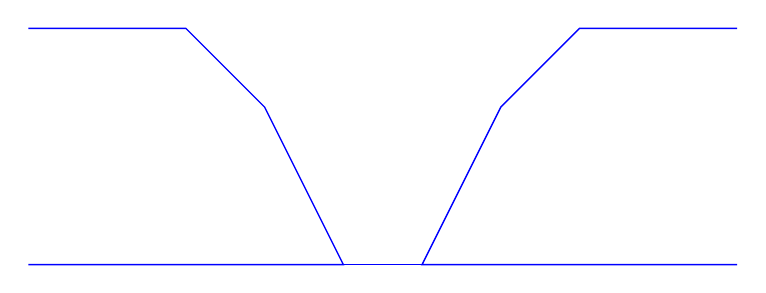
\begin{tikzpicture}
        \draw[line width=0.5,color=blue] (0,0)--(4,0)--(3,2)--(2,3)--(0,3);
        \draw[line width=0.5,color=blue] (9,0)--(5,0)--(6,2)--(7,3)--(9,3);
        \draw[line width=0.5,color=blue] (4,0)--(5,0);
    \end{tikzpicture}
    \caption{Possible shape interpretation of the volumetric isotherms of membrane 295a for a single pore. If the interpretation were correct, an incontinuoutity ?? of the anodizing current could be the reason for the change in funnelling.}
    \label{fig:weird-funnelling}
\end{figure}
\end{document}
